\section{Response Generation Module}

Fig.~\ref{fig:ResponseStrategy} gives \emph{TeenChat}'s response strategies
based on  user's sentence type and the detected result \texttt{(c.Stress,c.Category, c.SubCategory)}.

\noindent [\textbf{Case 1}] Stress being detected (\texttt{c.Stress==1})

\noindent (1) For a user's \texttt{declarative sentence} or \texttt{rhetorical question}, \emph{TeenChat} selects an answer from the \emph{local knowledge base}, which accommodates abundant of positive response sentences in different categories/sub-categories to comfort, encourage, or guide stressful users.

\noindent (2) For a user's \texttt{interrogative question}, \emph{TeenChat} goes to one of the largest Chinese Q\&A community \emph{Baidu Knows} to match the question with the given answer. Let $Q_u$ be the user's input question, and $Q_b$ be the closest question found in the Baidu Knows. If their matching degree $MatchDegree(Q_u,Q_b)$ is over a certain threshold $\theta$, and meanwhile $Q_b$'s corresponding answer has been adopted or agreed by at least one person, \emph{TeenChat} will return $Q_b$'s best answer to the user. Otherwise, \emph{TeenChat} will search the \emph{local knowledge base} and return a general positive answer, or just a joke to cheer up the user.
\begin{figure}
\begin{minipage}{\textwidth}
\centering
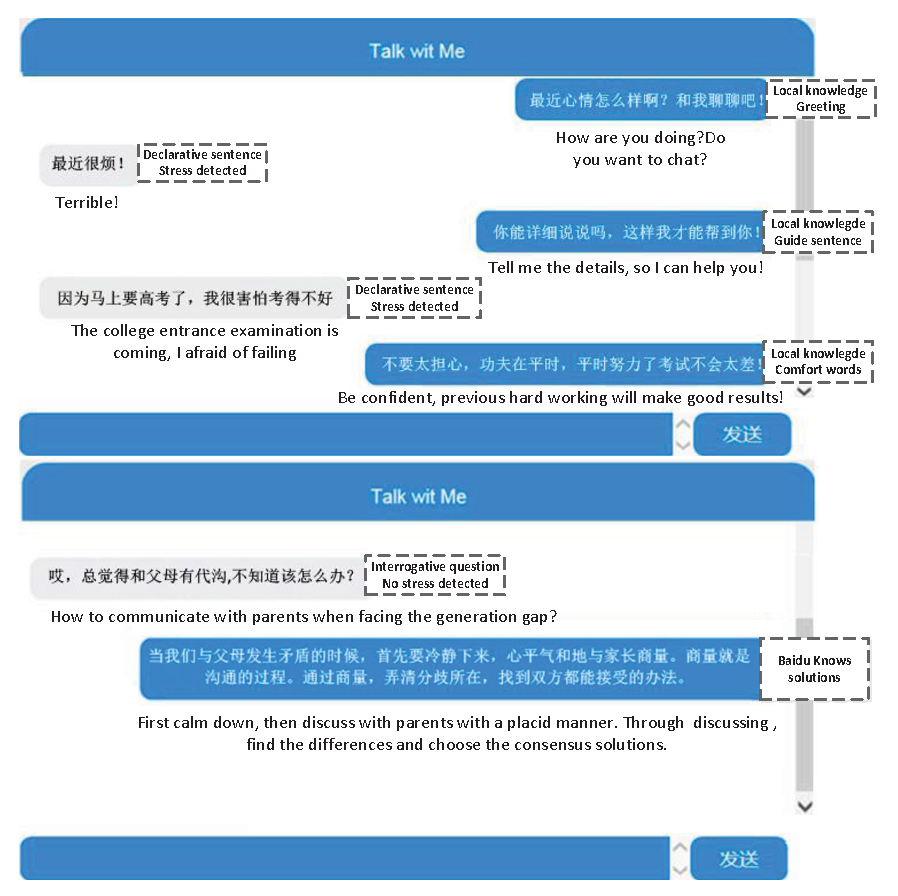
\includegraphics[height=8.8cm]{figs/Dialogexample.eps}
\caption{\emph{TeenChat} response examples of two topic categories}
\end{minipage}
\label{fig:example}
\end{figure}
The matching degree $MatchDegree$$(Q_u$,$Q_b)$ is computed based on the \emph{effective
node pairs} in the $Q_u$'s and $Q_b$'s linguistic dependence trees~\cite{36li2003}.
An \emph{effective node pair} is a node pair $(n_1,n_2)$, where $n_1$ is the core root node, $n_2$ is the direct child node of $n_1$, and $n_2$ represents a verb, noun, or adjective word. Given two effective node pairs $u=(u_1,u_2)$ and $b=(b_1,b_2)$, we define their similarity as:
\[sim(u,b)=sim((u_1,u_2),(b_1,b_2)) = \left\{ \begin{array}{ll}
1   & \mbox{if $(u_1==b_1) \wedge (u_2==b_2)$} \\
0.5 & \mbox{else if $(u_1==b_1) \wedge (u_2 \neq b_2)$} \\
0   & \mbox{otherwise}
\end{array}
\right. \]

Let $E(Q_u)$ and $E(Q_b)$ denote the set of effective node pairs in the $Q_u$'s and $Q_b$'s linguistic dependence trees, respectively.
Considering nodes' semantical equivalence, we replace any two nodes (one in $E(Q_u)$ and the other in $E(Q_b)$) with their
sememe in Hownet (if existing) to ensure nodes' similarity as much as possible. The obtained equivalent effective node sets are denoted as $E^*(Q_u)$ and $E^*(Q_b)$, respectively.
We have
$MatchDegree(Q_u,Q_b)=$
$\alpha ~ SIM(E(Q_u),E(Q_b))+$
$(1-\alpha) ~ SIM(E^*(Q_u),E^*(Q_b))$,
where $\alpha=0.5$,\\
$SIM(E(Q_u),E(Q_b))=\frac{\sum_{u \in E(Q_u)}~\sum_{b \in E(Q_b)}~sim(u,b)}{Max \{|E(Q_u)|, |E(Q_b)|\}}$, and \\
$SIM(E^*(Q_u),E^*(Q_b))=\frac{\sum_{u^* \in E^*(Q_u)}~\sum_{b^* \in E^*(Q_b)}~sim(u^*,b^*)}{Max \{|E^*(Q_u)|, |E^*(Q_b)|\}}$.

\noindent [\textbf{Case 2}] No stress being detected (\texttt{c.Stress==0})

\noindent (1) For a user's \texttt{interrogative question}, the answering is the same as the one in \emph{Case 1} (2).

\noindent (2) For a user's \texttt{non-interrogative question} input, \emph{TeenChat} goes to the open Simsimi repository~\cite{30SIMSIMI}, which provides public API for developers to establish their own chatting robot.

Fig.$4$ shows some example responses about study and interpersonal skills.

